\section{Über die GAF}

\subsection{\ldots{} dieses Heft}

Bei der ganzen Informationsflut, die in der ersten Unizeit auf dich
einstürzt, hoffen wir dir mit unserem \emph{Ersti-Einstein} einen
kleinen Ratgeber an die Hand zu geben.  Der Ersti-Einstein bündelt
Wichtiges, erklärt dir Nichtoffensichtliches, und versucht bei vielen
Problemen zumindest erste Lösungsansätze zu bieten.

Da wir nicht mehr alle Probleme, die ein Ersti hat, nachvollziehen
können, und jedes Jahr neue Probleme gefunden werden, würden wir uns
freuen, wenn du uns fehlende Informationen unter
\mail{einstein@fs.lmu.de} mitteilst.


\subsection{weg damit!}

Wir sind die GAF -- Gruppe Aktiver Fachschaftika -- ein
Zusammenschluss der Fachschaften der Fachbereiche
Mathematik,
Physik
und Informatik (also auch Wirtschaftsmathe, Medieninfo und
Meteorologie), sowie den dazugehörigen Lehramtsstudiengängen.

\paragraph{Was ist eine Fachschaft?}

Eine Fachschaft sind alle Studenten in einem Studiengang, das heißt die Fachschaft Physik besteht zum Beispiel aus \emph{allen} Studenten (ob ihr wollt oder nicht), die in Physik eingeschrieben sind.

Wenn man von \emph{der Fachschaft} spricht, meint man normalerweise die Aktiven,
zum Beispiel die Organisatoren der O-Phase.

\paragraph{Was macht die Fachschaft?}
\begin{itemize}
\item Repräsentation studentischer Interessen auf allen Ebenen, d.h. in Universitätsgremien z.B. dem Fakultätsrat, der Studiengebührenkommission oder Berufungskommissionen für neue Professoren \ldots
\item Verwaltung alter Klausuren, Prüfungsprotokolle und allem Anderen, was beim Studium hilft.
\item Information (O-Phase) und Beratung. Wenn du Fragen hast und nicht mal weißt, wen du fragen sollst, frag' uns.
\item Bespaßung: Wir organisieren Partys und andere Aktionen (Lange Nacht der Uni, Fakultätsfest, \ldots), damit auch der soziale Aspekt an der Uni nicht zu kurz kommt.
\item Anlaufstelle für Fragen aller Art; Sammeln von Meinungen für die Fakultät und Informationen aus der Fakultät, die wir an dich weiter leiten.
\end{itemize}

\paragraph{Wie machen die das?}
Die Fachschaft an sich bekommt Geld, das aber nur zum Nutzen der
Studenten eingesetzt werden darf, d.h. diejenigen, die in der
Fachschaft aktiv sind, tun dies ehrenamtlich und unentgeltlich.

\clearpage

\paragraph{Ich will mitmachen! Wie?}\label{mitmachen}\hfill\\

Komm einfach vorbei:
\begin{itemize}
	\item ins Fachschaftszimmer (Theresienstr., B037)
	\item zur Fachschaftssitzung (Termine unter \url{gaf.fs.lmu.de/wir/fachschaftssitzung})
\end{itemize}
oder sprich uns bei der O-Phase an.


\paragraph{Wie kann ich euch erreichen?}\label{gafKontakt}\hfill\\[1em]
%XXX To do: seperate Box/ optisch aufwerten
\begin{tabular}{ l l l l }
Telefon&089 / 2180\emd{}4382\\
Telefax&089 / 2180\emd{}4391\\
&\\
&\mail{gaf@fs.lmu.de}\\
&\mail{einstein@fs.lmu.de}\\
&\mail{gumbel@fs.lmu.de}\\
&\\
&\url{gaf.fs.lmu.de}\\
&\url{facebook.com/gaflmu}\\
&\\
IRC & \url{#gaf} auf freenode
\end{tabular}

\paragraph{Andere Fachschaften}
\begin{itemize}
	\item \textbf{Medieninformatik:} \url{mi.fs.lmu.de} und \url{facebook.com/FS.Medieninformatik.LMU}
	\item \textbf{Bioinformatik:} \url{www.bioinformatik-muenchen.com/bioinfocom/fachschaft/}
	\item \textbf{Meteorologie:} \url{www.meteo.physik.lmu.de/~studmet}
\end{itemize}

\skiptobottom
%XXX To do: neues Bild
\centerline{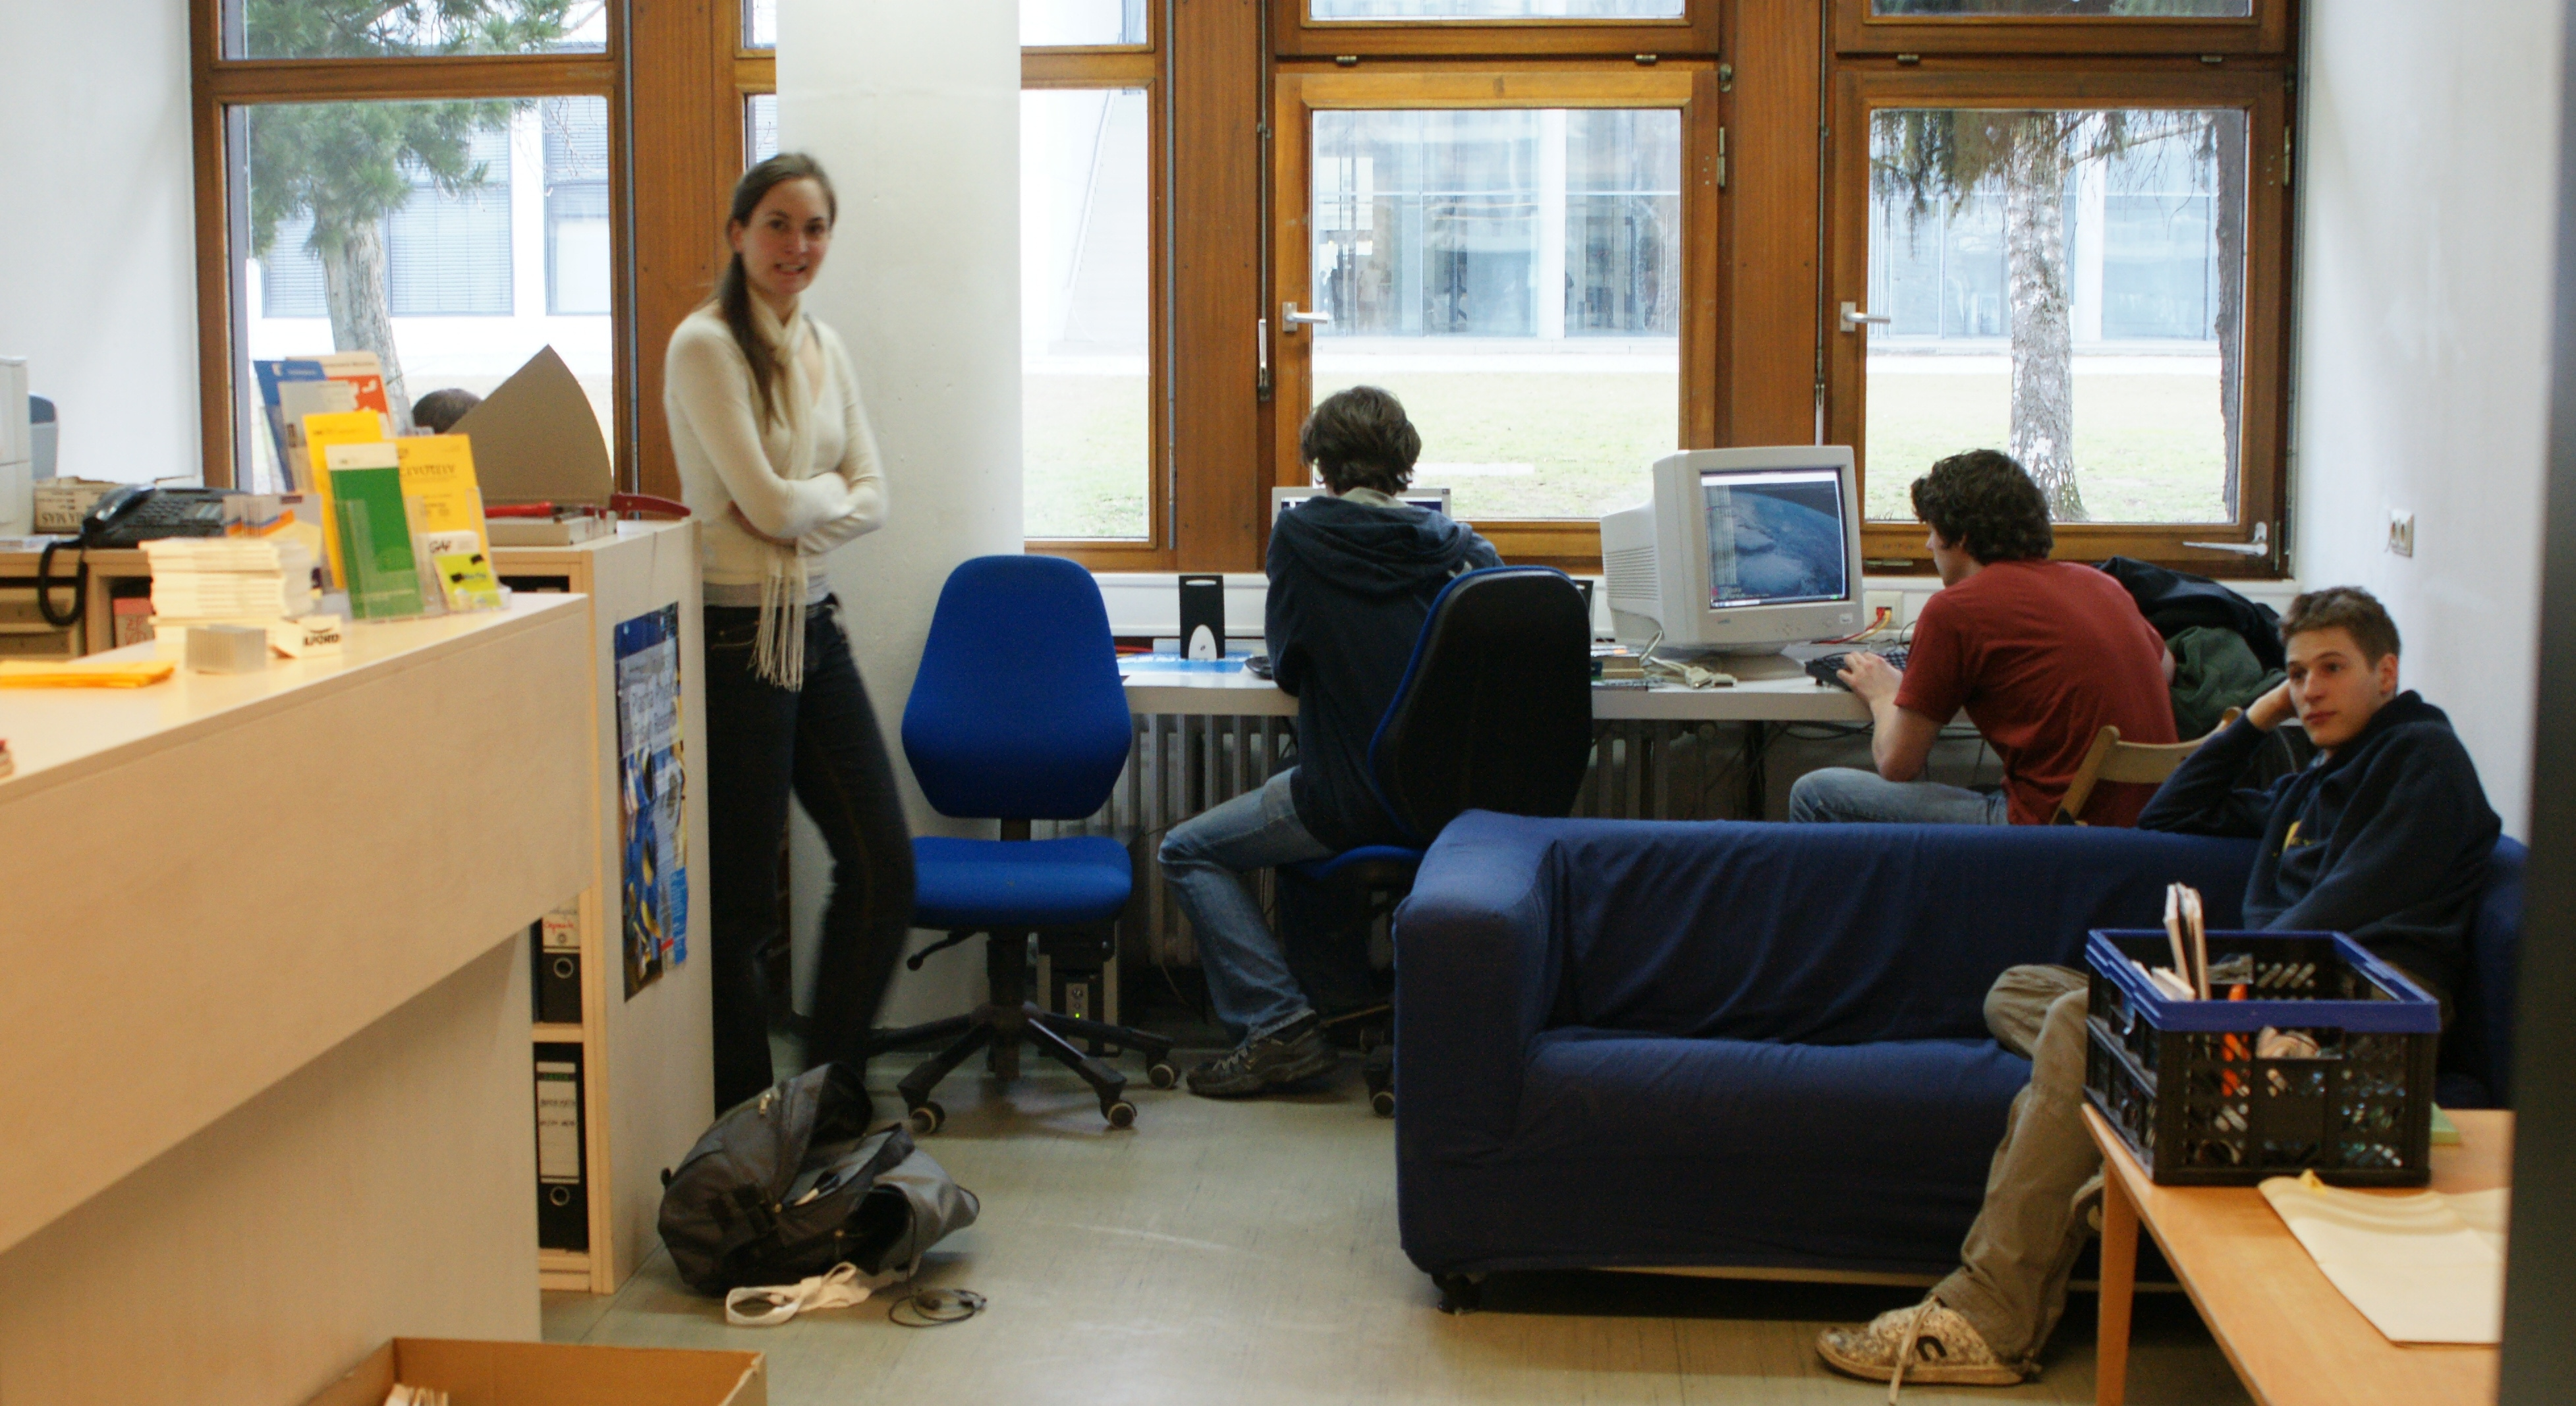
\includegraphics[width=0.8\textwidth]{aktive-fachschaft_print}}
